\documentclass[jou]{apa6}

\usepackage[american]{babel}

\usepackage{csquotes}
\usepackage[style=apa,sortcites=true,sorting=nyt,backend=biber]{biblatex}
\DeclareLanguageMapping{american}{american-apa}
\addbibresource{bibliography.bib}


%%%%%%%%%%%%%%%%%%%%%%%%%%%%%%%%%%%%%%%%
%% Discrete Structures
%% The start of RBS stuff
%%%%%%%%%%%%%%%%%%%%%%%%%%%%%%%%%%%%%%%%

% Working internal and external links in PDF
\usepackage{hyperref}
% Extra math symbols in LaTeX
\usepackage{amsmath}
\usepackage{gensymb}
\usepackage{amssymb}
% Enumerations with (a), (b), etc.
\usepackage{enumerate}
\usepackage{xcolor}

\let\OLDitemize\itemize
\renewcommand\itemize{\OLDitemize\addtolength{\itemsep}{-6pt}}

\usepackage{etoolbox}
\makeatletter
\preto{\@verbatim}{\topsep=3pt \partopsep=3pt }
\makeatother

% These sizes redefine APA for A4 paper size
\oddsidemargin 0.0in
\evensidemargin 0.0in
\textwidth 6.27in
\headheight 1.0in
\topmargin -24pt
\headheight 12pt
\headsep 12pt
\textheight 9.19in



\title{Sample Quiz 8}
\author{Discrete Structures, Spring 2020}
\affiliation{RBS}

\leftheader{Discrete Sample Quiz 8}

\abstract{%
}

%\keywords{}

\setlength\parindent{0pt}

\begin{document}

\thispagestyle{empty}

\twocolumn
{\Large Quiz 11 (Graphs)}

\vspace{4pt}
{\bf Question 1.}
Let $G = (V,E)$ be a graph, where $V$ is the set of all positive divisors of $144$ (including 
$1$ and $144$ itself). Two different vertices $d_1,d_2$ are connected by an edge iff one of the
numbers divides another ($d_1\,\mid\,d_2$ or $d_2\,\mid\,d_1$). 
Find the number of vertices $|V|$ and the number of edges $|E|$ in this graph.

Write two comma-separated integers.


\vspace{10pt}
{\bf Question 2.}
How long is the longest simple circuit in $W_{20}$? 
(A simple circuit is a circular path that may visit vertices multiple times, 
but does not contain any edge more than once.)

Write a positive integer. 




\vspace{10pt}
{\bf Question 3.}
Let $G$ be a planar connected graph with $60$ vertices, each vertex has degree $3$. 
How many regions are there in $G$?

Write a positive integer.



\vspace{10pt}
{\bf Question 4.} This is an adjacency matrix for some graph:
{\footnotesize
$$M_G = \left( 
\begin{array}{ccccccccc}
0 & 1 & 0 & 1 & 0 & 0 & 0 & 0 & 1 \\
1 & 0 & 1 & 1 & 1 & 0 & 0 & 0 & 0 \\
0 & 1 & 0 & 0 & 1 & 1 & 0 & 0 & 0 \\
1 & 1 & 0 & 0 & 1 & 0 & 1 & 0 & 0 \\
0 & 1 & 1 & 1 & 0 & 1 & 1 & 1 & 0 \\
0 & 0 & 1 & 0 & 1 & 0 & 0 & 1 & 1 \\
0 & 0 & 0 & 1 & 1 & 0 & 0 & 1 & 0 \\
0 & 0 & 0 & 0 & 1 & 1 & 1 & 0 & 1 \\
1 & 0 & 0 & 0 & 0 & 1 & 0 & 1 & 0 \\
\end{array} \right).$$
}

It is known that $G$ is a planar graph. Find the number of vertices $|V|$, 
number of edges $|E|$ and the number of regions $|R|$ for this graph. 

Write $3$ comma-separated integers.



\vspace{10pt}
{\bf Question 5 (Dudeney2016, Prob.434), ``536 Puzzles''.}
\begin{center}
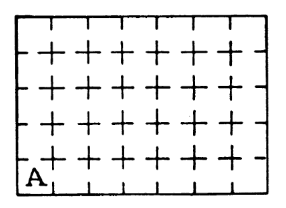
\includegraphics[width=1.5in]{prison-cells.png}
\end{center}
A prisoner currently is in the cell ``$A$''. He has to visit each 
prison cell no more than once and return 
back to the cell ``$A$''. What is the largest number of prison cells that
can be visited in this way?

Write a positive integer.

{\em Note.} You may also want to prove to yourself that the number is the largest possible.


\vspace{10pt}
{\bf Question 6}
There is a bipartite graph $G=(V,E)$ with exactly $|V| = 17$ vertices. (A graph is {\em bipartite}, if 
the set of vertices $V$ can be split into two parts $X$, $Y$ so that all edges are between a vertex in $X$ and a vertex in $Y$.)
Find the largest possible number of vertices in such a graph. 

Write a positive integer.
 

\vspace{10pt}
{\bf Question 7} Verify, if these statements are true. 
A simple undirected graph is called a {\em cubic} graph, 
if every vertex has degree $3$.\\
{\bf (A)} There exists a cubic graph with $7$ vertices.\\
{\bf (B)} There exists a cubic graph with $6$ vertices that is not isomorphic to $K_{3,3}$.\\
{\bf (C)} There exists a cubic graph with $8$ edges.

Write a sequence of 3 comma-separated letters (e.g.\ {\tt T,T,T} or {\tt F,F,F}).




\vspace{10pt}
{\bf Question 8.} Verify, if these statements are true:\\
{\bf (A)} There exists a simple directed graph with indegrees $0,1,2,4,5$ and outdegrees $0,3,3,3,3$. (A graph is {\em simple}, if
it is not a {\em multigraph} \textendash{} there is no more than one edge $(u,v)$ for any vertices $u,v$.)\\
{\bf (B)} There exists a connected undirected simple planar graph with $5$ regions and $8$ vertices, each vertex has degree $3$.\\
{\bf (C)} There exists a connected undirected simple planar graph with $8$ regions and $6$ vertices, each region is surrounded 
with $3$ edges.

Write a sequence of 3 comma-separated letters (e.g.\ {\tt T,T,T} or {\tt F,F,F}).



\vspace{10pt}
{\bf Question 9.}
Use Dijkstra’s Algorithm to find the shortest paths from the source vertex $s$ 
to all other vertices $t,x,y,z$. The length of a path is obtained by adding the 
weights of the directed edges.
\begin{center}
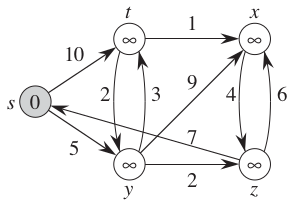
\includegraphics[width=1.8in]{dijkstra.png}
\end{center}

Write $4$ comma-separated numbers \textendash{} the shortest paths 
to the vertices $t,x,y,z$ respectively.

{\em Note.} Dijkstra's algorithm (Rosen2019, p.747) initializes the set of vertices $S$ that we 
know the shortest paths to (initially it only contains the 
source vertex $S = \{ s \}$; 
the distance from $s$ to itself is $0$; initialize the distances to 
all the other vertices to $\infty$). At every step consider all the edges that 
go from the set $S$ to $\overline{S}$, i.e. to the vertices where we still 
do not know the shortest paths. Update all the shortest paths (if crossing from 
the set $S$ to $\overline{S}$ finds a shorter path than $\infty$ or the currently 
known minimum length, then decrease the estimate for this vertex). 
Finally, add the minimum vertex from $\overline{S}$ to $S$. Repeat the steps
until all vertices are added to $S$ and all the shortest path estimates have 
reached their smallest values.





\vspace{10pt}
{\bf Question 10 (Dudeney2016, Prob.423), ``536 Puzzles''.}
A man starting from the town $A$, has to inspect all the roads
shown from town to town. Their respective lengths, $13$, $12$, and $5$
miles are all shown. What is the shortest possible route he can adopt, 
ending his journey wherever he likes?
\begin{center}
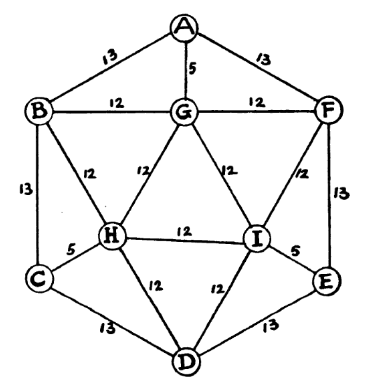
\includegraphics[width=2in]{path-with-repetitions.png}
\end{center}

Write an integer \textendash{} the length of the shortest route.

{\em Note.} This graph obviously has no Euler path (since there
are more than $2$ vertices with odd degrees). The problem is to 
find a path that is likely {\bf not} simple 
(uses the same edge several times), 
but that includes every edge shown and the total of weights is minimal. 





\vspace{10pt}
{\bf Question 11}\\
Somebody placed $24$ chess rooks on a $8 \times 8$ chessboard as shown in the picture 
(each horizontal and each vertical has exactly $3$ rooks). 
\begin{center}
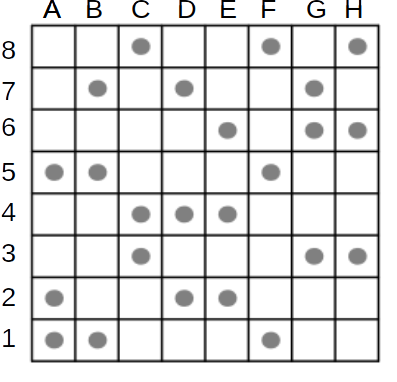
\includegraphics[width=1.5in]{quiz11/rooks.png}
\end{center}
We imagine that this chess-board defines a bipartite graph between the  
set of all verticals $X= \{ A,B,C,D,E,F,G,H \}$ and the set of all 
horizontals $Y= \{ 1,2,3,4,5,6,7,8 \}$. Any rook defines an edge between these two sets. 
For example, the rook $C8$ defines an edge $(C,8)$. 

Find a subset of verticals $V \subseteq X$ such that $|V|=3$, but
the neighbor set has size $|N(V)| = 5$.

Write $3$ comma-separated letters in your answer (the vertices from $V$). It is 
sufficient to write just one possible answer, if there are many.

\vspace{10pt}
{\em Note 1.} For example, the answer $\textcolor{blue}{\mathtt{F,G,H}}$ does not work, 
since the set of vertices $\{ \mathtt{F},\mathtt{G},\mathtt{H} \} \subseteq X$ 
is neighboring with a set of six vertices
$\{ 1,3,5,6,7,8 \} \subseteq Y$, i.e. the rooks on these three verticals
attack six horizontals, but not five.

{\em Note 2.} For the condition of the Hall's marriage theorem we need the inequality $|V| \leq |N(V)|$ 
for {\bf every} $V \subseteq X$. You could prove to yourself that it is always satisfied
(also for all the other placements of $24$ rooks where each horizontal and each 
vertical has $3$ rooks).\\
{\em Note 3.} Interpret for yourself what does a ``perfect matching'' between the sets
$X$ and $Y$ mean in this subject-area with a chessboard and rooks.




\end{document}

